\documentclass{ximera}
\author{Jim Talamo and Bart Snapp}
\newcommand{\RR}{\mathbb R}
\renewcommand{\d}{\,d}
\newcommand{\dd}[2][]{\frac{d #1}{d #2}}
\renewcommand{\l}{\ell}
\newcommand{\ddx}{\frac{d}{dx}}
\newcommand{\dfn}{\textbf}
\newcommand{\eval}[1]{\bigg[ #1 \bigg]}


\outcome{Define a sequence.}
\outcome{Write the first several terms of a sequence using an explicit formula.}
\outcome{Write the first several terms of a sequence using a recurrence
  relation.}
\outcome{Find an explicit formula for a sequence given recursively.}
\outcome{Find a recurrence relation for a sequence given explicitly.}

\title[Dig-In:]{Sequences}

\begin{document}
\begin{abstract}
  A sequence is an ordered list.
\end{abstract}
\maketitle


Let's get to the heart of the matter:

\begin{definition}
  A \dfn{sequence} is an ordered list of numbers.
\end{definition}

For example, here is a sequence:
\[
1,1, 2, 3, 5, 8, 13, 21, \ldots
\]
Here is another sequence:

\[
e, 3\pi, \arctan(27), \frac{1}{42}, \ldots
\]


Note that numbers in the list can repeat.  The dots ``\ldots'' signify that the list keeps
going, and going...and going forever.  We often ant to refer to a specific term in this list, so we introduce some standard notation:
%want a notation environment
\begin{definition} The notation:  $\left\{a_n\right\}_{n=1}$ will be used to denote the following ordered list of numbers:

\[
a_1, a_2,  a_3, \ldots,
\]
\end{definition}

The subscript in the above notation is called the \emph{index} and describes how we reference the first term.  In general, we like to index sequences starting at $n=0$ or $n=1$, but would like to have the freedom to make other choices should it be convenient.  Thus, there is no unique way to describe a given list of numbers; for example, for the sequence:

\[
1,1, 2, 3, 5, 8, 13, 21, \ldots
\]
we could define this by $\left\{a_n\right\}_{n=1}$, where $a_1=1$, $a_2=1$, $a_3=2$, etc or by  $\left\{b_n\right\}_{b=3}$, where $b_3=1$, $b_4=1$, $b_5=2$, etc.

\begin{remark}
Many authors denote sequences using other conventions.  Some other common notations you may see are: 

\begin{align*}
  &a_n = 2n+3, n \geq 1   \\
  & \left(a_n\right)_{n \in \N}, \\
  & \left\{a_n\right\}_{n=1}^\infty, \\
  & \left\{f(n)\right\}_{n=1}^\infty, \quad \text{or} \\
  & \left(f(n)\right)_{n \in \N},
\end{align*}
where $\N = \{1,2,3, \ldots \}$ denotes the set of natural  numbers. In this text, we will usually write $\left\{a_n\right\}$ if we want to speak of the sequence as a whole and we will write $a_n$ if we are referring to a specific element, or ``term'', in the sequence.

\end{remark}



\begin{question}
  Consider the sequence
  \[
  1, 2, 4, 8, 16, \dots.
  \]
  What number comes next?
  \begin{multipleChoice}
    \choice{$32$}
    \choice{$31$}
    \choice{$18$}
    \choice[correct]{there is no way to know}
  \end{multipleChoice}

While there seems to be a pattern, without explicitly listing more terms (or giving a rule that defines the successive terms), it's impossible to establish what the next term is! 

\end{question}

In fact, here are two different sequences whose first 5 terms are the same as the example above:

\begin{example}
  Let $a_n = 2^{n-1}$.  Write down $a_1$, $a_2$, $a_3$, $a_4$, $a_5$, and
  $a_6$.
  \begin{explanation}
    Use the formula to see:
    \begin{align*}
      a_1 &= \answer[given]{1} & a_2 &= \answer[given]{2} & 
      a_3 &= \answer[given]{4} & 
      a_4 &= \answer[given]{8} & 
      a_5 &= \answer[given]{16} & 
      a_6 &= \answer[given]{32}
    \end{align*}
  \end{explanation}
\end{example}


\begin{example}
  Consider a circle with $n$ points on it. Let $b_n$ be the maximum
  number of regions produced by connecting these points with
  chords. Write down $b_1$, $b_2$, $b_3$, $b_4$, $b_5$, and $b_6$.
  \begin{explanation}
    There is only one way to solve this problem: start drawing
    pictures and counting regions.
    \begin{itemize}
      \item \begin{tikzpicture}[framed,scale=1,baseline=-1ex]      
            \tkzDefPoint(0,0){O} 
            \tkzDefPoint(1,0){A} 
            \tkzDrawCircle[color=penColor,very thick](O,A)
            \tkzDrawPoint[color=penColor,fill=penColor](A)
      \end{tikzpicture} We see that $b_1 = \answer[given]{1}$
      \item \begin{tikzpicture}[framed,scale=1,baseline=-1ex]      
            \tkzDefPoint(0,0){O} 
            \tkzDefPoint(1,0){A} 
            \tkzDefPoint(-1,0){B}
            \tkzDrawCircle[color=penColor,very thick](O,A)
            \tkzDrawPoint[color=penColor,fill=penColor](A)
            \tkzDrawPoint[color=penColor,fill=penColor](B)
            \tkzDrawSegment[color=penColor](A,B)
      \end{tikzpicture} We see that $b_2 = \answer[given]{2}$
      \item \begin{tikzpicture}[framed,scale=1,baseline=-1ex]      
            \tkzDefPoint(0,0){O} 
            \tkzDefPoint(1,0){A} 
            \tkzDefPoint(-.6,.8){B}
            \tkzDefPoint(-.6,-.8){C}
            \tkzDrawCircle[color=penColor,very thick](O,A)
            \tkzDrawPoint[color=penColor,fill=penColor](A)
            \tkzDrawPoint[color=penColor,fill=penColor](B)
            \tkzDrawPoint[color=penColor,fill=penColor](C)
            \tkzDrawSegment[color=penColor](A,B)
            \tkzDrawSegment[color=penColor](A,C)
            \tkzDrawSegment[color=penColor](B,C)
      \end{tikzpicture} We see that $b_3 = \answer[given]{4}$
      \item \begin{tikzpicture}[framed,scale=1,baseline=-1ex]      
            \tkzDefPoint(0,0){O} 
            \tkzDefPoint(.6,.8){A} 
            \tkzDefPoint(-.6,.8){B}
            \tkzDefPoint(-.6,-.8){C}
            \tkzDefPoint(.6,-.8){D}
            \tkzDrawCircle[color=penColor,very thick](O,A)
            \tkzDrawPoint[color=penColor,fill=penColor](A)
            \tkzDrawPoint[color=penColor,fill=penColor](B)
            \tkzDrawPoint[color=penColor,fill=penColor](C)
            \tkzDrawPoint[color=penColor,fill=penColor](D)
            \tkzDrawSegment[color=penColor](A,B)
            \tkzDrawSegment[color=penColor](A,C)
            \tkzDrawSegment[color=penColor](A,D)
            \tkzDrawSegment[color=penColor](B,C)
            \tkzDrawSegment[color=penColor](B,D)
            \tkzDrawSegment[color=penColor](C,D)
      \end{tikzpicture} We see that $b_4 = \answer[given]{8}$
        \item \begin{tikzpicture}[framed,scale=1,baseline=-1ex]      
            \tkzDefPoint(0,0){O} 
            \tkzDefPoint(1,0){A} 
            \tkzDefPoint(.27,.96){B}
            \tkzDefPoint(-.8,.6){C}
            \tkzDefPoint(-.8,-.6){D}
            \tkzDefPoint(.33,-.95){E}
            \tkzDrawCircle[color=penColor,very thick](O,A)
            \tkzDrawPoint[color=penColor,fill=penColor](A)
            \tkzDrawPoint[color=penColor,fill=penColor](B)
            \tkzDrawPoint[color=penColor,fill=penColor](C)
            \tkzDrawPoint[color=penColor,fill=penColor](D)
            \tkzDrawPoint[color=penColor,fill=penColor](E)
            \tkzDrawSegment[color=penColor](A,B)
            \tkzDrawSegment[color=penColor](A,C)
            \tkzDrawSegment[color=penColor](A,D)
            \tkzDrawSegment[color=penColor](A,E)
            \tkzDrawSegment[color=penColor](B,C)
            \tkzDrawSegment[color=penColor](B,D)
            \tkzDrawSegment[color=penColor](B,E)
            \tkzDrawSegment[color=penColor](C,D)
            \tkzDrawSegment[color=penColor](C,E)
            \tkzDrawSegment[color=penColor](D,E)
        \end{tikzpicture} We see that $b_5 = \answer[given]{16}$
        \item \begin{tikzpicture}[framed,scale=1,baseline=-1ex]      
            \tkzDefPoint(0,0){O} 
            \tkzDefPoint(1,0){A} 
            \tkzDefPoint(0,1){B}
            \tkzDefPoint(-.8,.6){C}
            \tkzDefPoint(-.8,-.6){D}
            \tkzDefPoint(0,-1){E}
            \tkzDefPoint(.7,-.71){F}
            \tkzDrawCircle[color=penColor,very thick](O,A)
            \tkzDrawPoint[color=penColor,fill=penColor](A)
            \tkzDrawPoint[color=penColor,fill=penColor](B)
            \tkzDrawPoint[color=penColor,fill=penColor](C)
            \tkzDrawPoint[color=penColor,fill=penColor](D)
            \tkzDrawPoint[color=penColor,fill=penColor](E)
            \tkzDrawPoint[color=penColor,fill=penColor](F)
            \tkzDrawSegment[color=penColor](A,B)
            \tkzDrawSegment[color=penColor](A,C)
            \tkzDrawSegment[color=penColor](A,D)
            \tkzDrawSegment[color=penColor](A,E)
            \tkzDrawSegment[color=penColor](A,F)
            \tkzDrawSegment[color=penColor](B,C)
            \tkzDrawSegment[color=penColor](B,D)
            \tkzDrawSegment[color=penColor](B,E)
            \tkzDrawSegment[color=penColor](B,F)
            \tkzDrawSegment[color=penColor](C,D)
            \tkzDrawSegment[color=penColor](C,E)
            \tkzDrawSegment[color=penColor](C,F)
            \tkzDrawSegment[color=penColor](D,E)
            \tkzDrawSegment[color=penColor](D,F)
            \tkzDrawSegment[color=penColor](E,F)
            \end{tikzpicture} We see that $b_6 = \answer[given]{31}$
    \end{itemize}
    While we have made no real argument that these are the maximum
    number of regions, we believe that if the young mathematician draws
    more pictures they will be convinced.
  \end{explanation}
\end{example}


From the two sequences we've just considered, the method of ``finding a pattern'' is \textbf{not enough} when dealing with sequences unless you understand exactly how the sequence was produced.   However, having to define each term explicitly is quite cumbersome.  In general, we want to define a sequence by specifying a rules that will allow us to write down any term that we want.  There are two important ways that are generally used to describe a sequence:

\section{Two common methods of representing sequences}

\begin{definition}
We say that a sequence $\{a_n\}_{n=1}$ is described by an \dfn{explicit formula} the term $a_n$ is expressed in terms of $n$ only.
\end{definition}

Just as real-valued functions were usually expressed by a formula, we
will most often encounter sequences that can be expressed by a
formula.  We say that such sequences are defined \textit{explicitly}, 
or that we have an explicit formula for the sequence.

\begin{example}
Suppose $\{a_n\}_{n=1}$ is a sequence defined by the formula $a_n = 2n+3$.  Write down $a_1$, $a_2$, $a_3$, $a_4$, and $a_5$.

  \begin{explanation}
    By substituting $n=1, 2, 3, 4$ and $5$ into the formula above, we see:
    \begin{align*}
      a_1 &= \answer[given]{5} & 
      a_2 &= \answer[given]{7} & 
      a_3 &= \answer[given]{9} & 
      a_4 &= \answer[given]{11} & 
      a_5 &= \answer[given]{13} 
    \end{align*}
    
Thus, the rule $a_n = 2n+3, n \geq 1$ thus generates the ordered list:

\[
5,7,9,11,13, \dots
\]   

and we can use pattern recognition to generate more terms since we have a rule that defines the pattern.
  \end{explanation}
  
\end{example}

%Other examples are easy to cook up, as now we can use \textit{many} previously-encountered functions
%to define sequences.  For instance:
%
%\begin{align*}
%  a_i &=\frac{i}{i+1}, \\
%  b_n &=\frac{1}{2^n}, \\
%  c_j &=\sin(j\pi/6), \text{ or} \\
%  d_k &=\frac{(k-1)(k+2)}{2^k}. 
%\end{align*}
%Frequently, the formulas we use to define sequences will also make sense as
%functions with domain $\R$ or $\N$.  Occasionally, such a 
%formula will make sense only for integers (positive, zero, and
%negative whole numbers).

\begin{warning}
  A common misconception is to confuse the sequence with the rule for
  generating the sequence.  The sequences $\{a_n\}$ and $\{b_n\}$ given by
  the rules $a_n = (-1)^n$ and $b_n = \cos (\pi \cdot n)$ are, despite
  appearances, different rules which give rise to the \textit{same}
  sequence.  These are just different names for the same object!
\end{warning}


\begin{definition}
  Suppose $(a_n)$ and $(b_n)$ are sequences starting at $1$.  These
  sequences are \dfn{equal}\index{sequence!equality} if for all
  natural numbers $n$, we have $a_n = b_n$.

  More generally, two sequences $(a_n)$ and $(b_n)$ are
  \dfn{equal} if they have the same initial index $N$  and for
  every integer $n \geq N$, the $n$th terms have the same value, that is,
  \[
  a_n = b_n \quad \text{for all $n \geq N$.}
  \]
\end{definition}
%Put another way, sequences are the same if they have the same set of
%valid indices, and produce the same real numbers for each of those
%indices---regardless of whether the given ``rules'' or procedures for
%computing those sequences resemble each other in any way.

\begin{definition}
We say that a sequence $\{a_n\}_{n=1}$ is described by a \dfn{recursive formula} if the term $a_n$ is expressed in terms of $n$ and at least one of the previous terms in the sequence.
\end{definition}

We start by defining the first few elements of the sequence, and then describe how later elements are computed in terms of previous elements.

\begin{example}
 Suppose that $\{a_n\}_{n=1}$ is a sequence defined by the formula $a_n = a_{n-1}+2$, where $a_1 = 5$.  Write down $a_2$, $a_3$, $a_4$, and $a_5$.
 
 \begin{explanation}
 Substituting in $n=2$ gives:
 
 \[
 a_2 = a_{\answer[given]{1}}+2 = \answer[given]{5}+2 = \answer[given]{7}
 \]
 We can now plug in $n=3$ and use the previous result for $a_2$ to find $a_3$:
  \[
 a_3 = a_{\answer[given]{2}}+2 = \answer[given]{7}+2 = \answer[given]{9}
 \]
 Continuing, we find $a_4 = \answer[given]{11}$ and $a_5 = \answer[given]{13}$.
 
 Thus, the rule $a_n = 2n+3, n \geq 1$ thus generates the ordered list:

\[
5,7,9,11,13, \dots
\]   

 \end{explanation}
\end{example}

Note that both the explicit formula and recursive formula in the previous examples seem to generate the same list of numbers.  By writing out more and more terms, the young mathematician will find that it indeed seems like these seemingly different rules generate the same sequence!  

  \begin{remark}
  The idea of ``recognizing a pattern" and using it to generate more terms for the above example can be made more mathematically explicit through the notion of \emph{mathematical induction}.  The young mathematician may hypothesize that based on the pattern in the recursive formula:
  
  \[
  a_n = a_{n-1}+2, a_1 = 5
  \]
  
  the explicit rule $a_n = 2n+3$ for $n \geq 1$ generates the same sequence, and may prove beyond doubt that this is indeed the case by using induction.  We leave it to the curious young mathematician to research and explore this idea further.
  \end{remark}
  
  
  
  
%%EXERCISE%%%
%\begin{example}
%Define a sequence recursively by
%\[
%a_1 = 1, \quad a_2 = 3, \quad a_3 = 10,
%\]
%and the rule that $a_n = a_{n-1} - a_{n-3}$.  Compute $a_5$.
%\begin{explanation}
%  First we compute $a_4$.  Substituting $4$ for $n$ in the recursive
%  rule $a_n = a_{n-1} - a_{n-3}$, we find
%  \begin{align*}
%  a_4 &= a_{\answer[given]{4}-1} - a_{\answer[given]{4}-3} \\
%  &= a_3 - a_1.
%  \end{align*}
%  But we have values for $a_3$ and $a_1$, namely $10$ and $1$,
%  respectively.  Therefore $a_4 = 10 - 1 = \answer[given]{9}$.  Now we
%  are in a position to compute $a_5$.  Substituting $5$ for $n$ in the
%  rule $a_n = a_{n-1} - a_{n-3}$, we find
%  \[
%  a_5 = a_{5-1} - a_{5-3} = a_4 - a_2.
%  \]
%  We just computed $a_4 = 9$; we were given $a_2 = 3$.  Therefore
%  \begin{align*}
%    a_5&= \answer[given]{9} - 3 \\
%    &= \answer[given]{6}.
%  \end{align*}
%\end{explanation}
%\end{example}



%%%MOVE TO EXERCISES%%%
%\begin{question}
%  Consider the sequence $a_{n}$ defined recursively by the
%  rule
%  \[
%  a_n = {a_{n-1}} {a_{n-2}} + 3 \, {a_{n-1}} - {a_{n-2}}
%  \]
%  and the facts that $a_0 = -3$ and $a_1 = 5$.  What is $a_4$?
%  
%    \begin{hint}
%      We have been told the first two terms of the sequence, namely $a_0 = -3$ and $a_1 = 5$.
%    \end{hint}
%    \begin{hint}
%      We also have a rule $a_n = {a_{n-1}} {a_{n-2}} + 3 \, {a_{n-1}} - {a_{n-2}}$ which lets us compute the third term $a_2$ using these first two terms $a_0$ and $a_1$.
%    \end{hint}
%    \begin{hint}
%      To compute $a_2$, we set $n = 2$ in the recursive rule $a_n = {a_{n-1}} {a_{n-2}} + 3 \, {a_{n-1}} - {a_{n-2}}$.  This gives us $a_2 = {a_{2-1}} {a_{2-2}} + 3 \, {a_{2-1}} - {a_{2-2}}$.
%    \end{hint}
%    \begin{hint}
%      Plugging $a_{2-1} = a_{1} = 5$ and $a_{2-2} = a_{0} = -3$ into the rule, we learn $a_2 = 3$.
%    \end{hint}
%    \begin{hint}
%      To compute $a_3$, we set $n = 3$ in the recursive rule $a_n = {a_{n-1}} {a_{n-2}} + 3 \, {a_{n-1}} - {a_{n-2}}$, giving $a_3 = {a_{3-1}} {a_{3-2}} + 3 \, {a_{3-1}} - {a_{3-2}}$.
%    \end{hint}
%    \begin{hint}
%      To evaluate that, we will have to know $a_{3-1} = a_{2}$, but we just found out that $a_{2} = 3$.
%    \end{hint}
%    \begin{hint}
%      Plugging $a_{3-1} = 3$ and $a_{3-2} = a_{1} = 5$ into the rule, we find $a_3 = 19$.
%    \end{hint}
%    \begin{hint}
%      To compute $a_4$, we set $n = 4$ in the recursive rule $a_n = {a_{n-1}} {a_{n-2}} + 3 \, {a_{n-1}} - {a_{n-2}}$, giving $a_4 = {a_{4-1}} {a_{4-2}} + 3 \, {a_{4-1}} - {a_{4-2}}$.
%    \end{hint}
%    \begin{hint}
%      To evaluate that, we will have to know $a_{4-1} = a_{3}$, but we just found out that $a_{3} = 19$.
%    \end{hint}
%    \begin{hint}
%      Plugging $a_{4-1} = 19$ and $a_{4-2} = a_{2} = 3$ into the rule, we learn $a_4 = 111$.
%    \end{hint}
%    \begin{hint}
%      So we conclude $a_4 = 111$.
%    \end{hint}
%    \begin{prompt}
%      \[
%      a_4 = \answer[given]{111}.
%      \]
%    \end{prompt}
%\end{question}






%\section{Arithmetic sequences}
%
%
%The first family we consider are the ``arithmetic'' sequences.  Here
%is a definition.
%
%%{Mathematically, the word \dfn{family}
%%  does not have an entirely precise definition; a family of things is
%%  a \dfn{collection} or a \dfn{set} of things, but family
%%  also has a connotation of some sort of relatedness.} 
%
%\begin{definition}
%  An \dfn{arithmetic sequence} (sometimes called an arithmetic
%  progression)\index{arithmetic progression} is a sequence where the
%  difference between subsequent elements is constant.
%\end{definition}
%
%
%\begin{example}
%  Here is an example of an arithmetic sequence.
%  \begin{image}
%  \begin{tikzpicture}[node distance=1.5cm]
%    \node (a1) {$-5$,};
%    \node (a2) [right of=a1] {$-1$,};
%    \node (a3) [right of=a2] {$3$,};
%    \node (a4) [right of=a3] {$7$,};
%    \node (a5) [right of=a4] {$11$,};
%    \node (a6) [right of=a5] {$\ldots$};
%
%    \path[->] (a1) edge [bend left=20] node[above]{$+4$} (a2);
%    \path[->] (a2) edge [bend left=20] node[above]{$+4$} (a3);
%    \path[->] (a3) edge [bend left=20] node[above]{$+4$} (a4);
%    \path[->] (a4) edge [bend left=20] node[above]{$+4$} (a5);
%    \path[->] (a5) edge [bend left=20] node[above]{$+4$} (a6);
%  \end{tikzpicture}
%  \end{image}
%  This sequence is given explicitly by the function $a_n=\answer[given]{4n-9}$,
%  or recursively by the rule $a_1 = \answer[given]{-5}$ and $a_{i+1} = a_i
%  + \answer[given]{4}$. The difference between subsequent elements in this sequence is always four.
%\end{example}
%
%An arithmetic sequence can also decrease as it progresses.
%
%\begin{example}
%  Here is an example of an arithmetic sequence.
%  \begin{image}
%  \begin{tikzpicture}[node distance=1.5cm]
%    \node (a1) {$17$,};
%    \node (a2) [right of=a1] {$15$,};
%    \node (a3) [right of=a2] {$13$,};
%    \node (a4) [right of=a3] {$11$,};
%    \node (a5) [right of=a4] {$9$,};
%    \node (a6) [right of=a5] {$\ldots$};
%
%    \path[->] (a1) edge [bend left=20] node[above]{$-2$} (a2);
%    \path[->] (a2) edge [bend left=20] node[above]{$-2$} (a3);
%    \path[->] (a3) edge [bend left=20] node[above]{$-2$} (a4);
%    \path[->] (a4) edge [bend left=20] node[above]{$-2$} (a5);
%    \path[->] (a5) edge [bend left=20] node[above]{$-2$} (a6);
%  \end{tikzpicture}
%  \end{image}
%  This sequence is given explicitly by the function $a_n=\answer[given]{-2n + 19}$, or
%  recursively by the rule $a_1 = \answer[given]{17}$ and $a_{i+1} = a_i +
%  \answer[given]{(-2)}$. The difference between any subsequent elements in this sequence is negative
%  two.
%\end{example}
%
%
%
%In general, an arithmetic sequence in which subsequent terms differ
%by $m$ can be written as
%\[
%a_n = m (n-1) + a_1.
%\]
%Alternatively, we could describe an arithmetic sequence recursively,
%by giving a starting value $a_1$, and using the rule that $a_{n} =
%a_{n-1} + m$.  You should check that this general statement holds for our 
%two previous examples!
%
%
%\begin{remark}
%Why are arithmetic sequences called \textit{arithmetic}?  Note that
%every term is the \dfn{arithmetic mean} or \dfn{average} of its two
%neighbors.  The arithmetic mean of two numbers $a$ and $b$ is defined
%to be $\frac{a+b}{2}$.
%\end{remark}
%
%
%
%\begin{question}
%  Which of the following sequences are arithmetic sequences for
%  $n=1,2,3,\dots$?
%  \begin{selectAll}
%    \choice[correct]{$a_n = -3n + 5$}
%    \choice{$a_n = -5\cdot 7^{n+4}$}
%    \choice[correct]{$a_n = 5$}
%    \choice{$a_n = \left(\frac{1}{3}\right)\cdot a_{n-1}$ where $a_1 = 10$}
%    \choice[correct]{$a_n = \frac{4n^2+n-14}{n+2}$}
%    \choice{$a_n = 2^{n\cdot \cos(2\pi n + \pi))}$} 
%    \choice{$a_n = \cos(\pi/2^n)$}
%    \choice{$a_n = \cos(\pi n -5)$}
%    \choice[correct]{$a_n = n\cdot \cos(2\pi n) +4$}
%  \end{selectAll}
%  \begin{hint}
%    Look for a common difference between successive elements in the sequence. 
%  \end{hint}
%\end{question}
%
%
%%\subsection{Arithmetic sequences in the wild}
%%BADBAD it would be good to have examples...
%
%
%\section{Geometric sequences}
%
%
%The second family of sequences we consider are ``geometric''
%sequences.
%
%\begin{definition}
%  A \dfn{geometric sequence} (sometimes called a geometric
%  progression)\index{geometric progression} is a sequence where the
%  ratio between subsequent elements is constant.
%\end{definition}
%
%\begin{example}
%  Here is an example of a geometric sequence:
%  \begin{image}
%    \begin{tikzpicture}[node distance=1.5cm]
%    \node (a1) {$10$,};
%    \node (a2) [right of=a1] {$30$,};
%    \node (a3) [right of=a2] {$90$,};
%    \node (a4) [right of=a3] {$270$,};
%    \node (a5) [right of=a4] {$810$,};
%    \node (a6) [right of=a5] {$\ldots$};
%
%    \path[->] (a1) edge [bend left=20] node[above] {$\times 3$} (a2);
%    \path[->] (a2) edge [bend left=20] node[above] {$\times 3$} (a3);
%    \path[->] (a3) edge [bend left=20] node[above] {$\times 3$} (a4);
%    \path[->] (a4) edge [bend left=20] node[above] {$\times 3$} (a5);
%    \path[->] (a5) edge [bend left=20] node[above] {$\times 3$} (a6);
%  \end{tikzpicture}
%  \end{image}
%  This sequence is given explicitly by the function $a_n=\answer[given]{10\cdot
%    3^{n-1}}$, or recursively by the rule $a_1 = \answer[given]{10}$ and
%  $a_{i+1} = \answer[given]{3}\cdot a_i$. The ratio between any subsequent elements of our sequence is three.
%\end{example}
%
%A geometric sequence can also decrease as it progresses.
%
%\begin{example}
%  Here is an example of a geometric sequence:
%  \begin{image}
%    \begin{tikzpicture}[node distance=1.5cm]
%    \node (a1) {$\frac{7}{5}$,};
%    \node (a2) [right of=a1] {$\frac{7}{10}$,};
%    \node (a3) [right of=a2] {$\frac{7}{20}$,};
%    \node (a4) [right of=a3] {$\frac{7}{40}$,};
%    \node (a5) [right of=a4] {$\frac{7}{80}$,};
%    \node (a6) [right of=a5] {$\ldots$};
%
%    \path[->] (a1) edge [bend left=20] node[above] {$\times\frac{1}{2}$} (a2);
%    \path[->] (a2) edge [bend left=20] node[above] {$\times\frac{1}{2}$} (a3);
%    \path[->] (a3) edge [bend left=20] node[above] {$\times\frac{1}{2}$} (a4);
%    \path[->] (a4) edge [bend left=20] node[above] {$\times\frac{1}{2}$} (a5);
%    \path[->] (a5) edge [bend left=20] node[above] {$\times\frac{1}{2}$} (a6);
%  \end{tikzpicture}
%  \end{image}
%  This sequence is given by the function $a_n=\answer[given]{\left(\frac{7}{5}\right)\cdot
%    \left(\frac{1}{2}\right)^{n-1}}$, or the recursive rule $a_1 = \answer[given]{\frac{7}{5}}$ and
%  $a_{i+1} = \answer[given]{\left(\frac{1}{2}\right)}\cdot a_i$. The ratio between subsequent terms 
%  of this sequence is always one half.
%\end{example}
%
%
%A geometric sequence can have a negative ratio between successive
%elements.
%
%\begin{example}
%  Here is an example of a geometric sequence:
%  \begin{image}
%    \begin{tikzpicture}[node distance=1.5cm]
%    \node (a1) {$\frac{3}{5}$,};
%    \node (a2) [right of=a1] {$\frac{-3}{25}$,};
%    \node (a3) [right of=a2] {$\frac{3}{125}$,};
%    \node (a4) [right of=a3] {$\frac{-3}{625}$,};
%    \node (a5) [right of=a4] {$\frac{3}{3125}$,};
%    \node (a6) [right of=a5] {$\ldots$};
%
%    \path[->] (a1) edge [bend left=20] node[above] {$\times\frac{-1}{5}$} (a2);
%    \path[->] (a2) edge [bend left=20] node[above] {$\times\frac{-1}{5}$} (a3);
%    \path[->] (a3) edge [bend left=20] node[above] {$\times\frac{-1}{5}$} (a4);
%    \path[->] (a4) edge [bend left=20] node[above] {$\times\frac{-1}{5}$} (a5);
%    \path[->] (a5) edge [bend left=20] node[above] {$\times\frac{-1}{5}$} (a6);
%  \end{tikzpicture}
%  \end{image}
%  This sequence is given by the function $a_n=\answer[given]{\left(\frac{3}{5}\right)\cdot
%    \left(\frac{-1}{5}\right)^{n-1}}$, or the recursive rule $a_1 = \answer[given]{\frac{3}{5}}$ and
%  $a_{i+1} = \answer[given]{\left(\frac{-1}{5}\right)}\cdot a_i$. The ratio between any successive terms is negative one fifth.  Notice that this sequence is different from many others that we've studied so far: the terms are alternately positive and negative.
%\end{example}
%
%
%
%In general, a geometric sequence in which the ratio between
%subsequent terms is $r$ can be written as
%\[
%a_n = a_1 \cdot r^{n-1}.
%\]
%Alternatively, we could describe a geometric sequence
%recursively, by giving a starting value $a_1$, and using the rule that
%$a_{n} = r \cdot a_{n-1}$.  As usual, you should check that these general 
%rules hold for the specific examples we've considered!
%
%\begin{remark}
%Why are geometric sequences called \textit{geometric}?  Note that
%every term is the \dfn{geometric mean} of its two neighbors.  The
%geometric mean of two numbers $a$ and $b$ is defined to be
%$\sqrt{ab}$.
%
%Of course, that raises another question: why is the geometric mean
%called \textit{geometric?}  One geometric interpretation of the
%geometric mean of $a$ and $b$ is this: the geometric mean is the side
%length of a square whose area is equal to that of the rectangle having
%side lengths $a$ and $b$.
%\end{remark}
%
%\begin{question}
%  Which of the following sequences are geometric sequences for
%  $n=1,2,3,\dots$?
%  \begin{selectAll}
%    \choice{$a_n = -3n + 5$}
%    \choice[correct]{$a_n = -5\cdot 7^{n+4}$}
%    \choice[correct]{$a_n = 5$}
%    \choice[correct]{$a_n = \left(\frac{1}{3}\right)\cdot a_{n-1}$ where $a_1 = 10$}
%    \choice{$a_n = \frac{4n^2+n-14}{n+2}$}
%    \choice[correct]{$a_n = 2^{n\cdot \cos(2\pi n + \pi))}$} 
%    \choice{$a_n = \cos(\pi/2^n)$}
%    \choice[correct]{$a_n = \cos(\pi n -5)$}
%    \choice{$a_n = n\cdot \cos(2\pi n) +4$}
%  \end{selectAll}
%  \begin{hint}
%    Look for a common ratio between successive elements in the sequence. 
%  \end{hint}
%\end{question}

\section{Generating new sequences from other sequences}

Once we have defined a given sequence, we can define new sequences using it.

\begin{example}
Suppose that $\{a_n\}_{n=1}$ is defined by the rule:

\[
a_n = 3n-1
\]

We are going to build new sequences from this one, so let's write out some terms in the sequence $\{a_n\}$:

    \begin{align*}
      a_1 &= \answer[given]{2} & 
      a_2 &= \answer[given]{5} & 
      a_3 &= \answer[given]{8} & 
      a_4 &= \answer[given]{11} & 
      a_5 &= \answer[given]{14}  & 
      a_6 &= \answer[given]{17} 
    \end{align*}

\begin{example}
Define a new sequence: $\{b_n\}_{n=1}$ by the rule:

\[
b_n = \frac{a_{n+1}}{a_n} 
\]
Write out the first five terms in this new sequence.

\begin{explanation}
Starting with $n=1$ we find:

\[      b_1 = \frac{a_{\answer{2}}}{a_{\answer{1}}} = \answer[given]{\frac{5}{2}}       \]
      
Continuing in the same way, we find:     
     \begin{align*}
      	b_2 &=  \answer[given]{\frac{8}{5}}  & 
	b_3 &= \answer[given]{\frac{11}{8}}  & 
	b_4 &= \answer[given]{\frac{14}{11}}  & 
	b_5 &=  \answer[given]{\frac{17}{14}}  & 
    \end{align*}
    
\end{explanation}
    
\end{example}

\begin{example}
Define another new sequence: $\{c_n\}_{n=1}$ by the rule:

\[
c_n = \sqrt[n]{a_n} 
\]
Write out the first five terms in this new sequence.

\begin{explanation}
Starting with $n=1$ we find:

\[      c_1 = \sqrt[1]{a_1} = \answer[given]{2}       \]
      
Continuing in the same way, we find:     
     \begin{align*}
      	c_2 &=  \answer[given]{\sqrt[2]{5}}  & 
	c_3 &= \answer[given]{\sqrt[3]{8}}   & 
	c_4 &= \answer[given]{\sqrt[4]{11}}   & 
	c_5 &=  \answer[given]{\sqrt[5]{14}}   & 
    \end{align*}
    
\end{explanation}
\end{example}

\begin{example}
Define another new sequence: $\{s_n\}_{n=1}$ by the rule:

\[
s_n = \sum_{k=1}^n a_k 
\]
Write out the first five terms in this new sequence.

Recall that the notation $\sum_{k=1}^n a_k$ is shorthand notation used to represent the sum: $a_1+a_2+\ldots a_n$



\begin{explanation}
Starting with $n=1$ we find:

\[      s_1 = a_1 = \answer[given]{2}       \]
      
Continuing in the same way, we find:     
     \begin{align*}
      	s_2 &=  a_1 +a_2 = \answer[given]{7}  \\ 
	s_3 &=  a_1 +a_2 + a_3 = \answer[given]{15}   \\ 
	s_4 &=  a_1 +a_2 +a_3 +a_4= \answer[given]{26}  \\ 
	s_5 &=  a_1 +a_2 +a_3+a_4+a_5= \answer[given]{40}    
    \end{align*}
Note that there are 2 ways to compute each of the terms above.  One way is to perform the explicit addition each time, but the clever young mathematician may notice that there is a faster way.  For instance, if we have already computed $s_3$, we may notice:

\begin{image}
  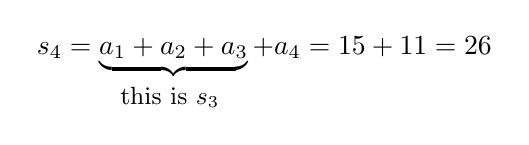
\begin{tikzpicture}
        \node at (0,0) {
          $s_4 = \underbrace{a_1+a_2+a_3} + a_4 = 15+11 =26$
        };
        \node at (-1.2,-.5) {\small{this is $s_3$}};
      \end{tikzpicture}
  \end{image}

The astute young mathematician may go as far as to notice that in general:

\begin{image}
  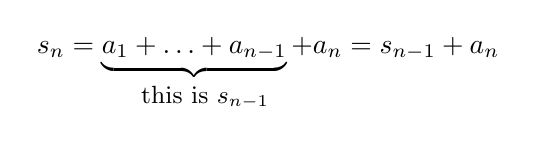
\begin{tikzpicture}
        \node at (0,0) {
          $s_n = \underbrace{a_1+\ldots+a_{n-1}} + a_n = s_{n-1} + a_n$
        };
        \node at (-.8,-.5) {\small{this is $s_{n-1}$}};
      \end{tikzpicture}
  \end{image}
so that in this example, where $a_n = 3n-1$, we have a recursive formula for $\{s_n\}_{n=1}$:

\[
s_n = s_{n-1} + (3n-1)
\]  

With more work, an explicit formula may also be developed:

\[
s_n = \frac{3n^2+n}{2}
\]
    
\end{explanation}
\end{example}   
\end{example}

The above sequences will all play an important role in the development that follows.  We will see how they arise in the context of answering a fundamental question introduced in the next section, but it is worth mentioning them now as new sequences that can be constructed from a given sequence!


%Let's start with a geometric interpretation.
%
%\begin{example}
%  Consider a unit square. Cut the square into two equal regions. Let
%  $a_1$ be the area of one of the regions. Cut the other region into
%  two equal regions and let $a_2$ be the area of one of these
%  regions. Continue on \textit{ad-infinitium}:
%  \begin{image}[2in]
%    \begin{tikzpicture}[scale=3]
%      \tkzDefPoint(0,0){A} 
%      \tkzDefPoint(1,0){B} 
%      \tkzDefPoint(1,1){C}
%      \tkzDefPoint(0,1){D}
%      \draw[penColor,very thick] (A)--(B)--(C)--(D)--cycle;
%
%      \tkzDefPoint(.5,1){D} 
%      \tkzDefPoint(.5,0){E} 
%      \draw[penColor,very thick] (D)--(E);
%
%      \tkzDefPoint(.5,.5){F} 
%      \tkzDefPoint(1,.5){G} 
%      \draw[penColor,very thick] (F)--(G);
%
%      \tkzDefPoint(.75,1){H} 
%      \tkzDefPoint(.75,.5){I} 
%      \draw[penColor,very thick] (H)--(I);
%
%      \tkzDefPoint(.75,.75){J} 
%      \tkzDefPoint(1,.75){K} 
%      \draw[penColor,very thick] (J)--(K);
%
%      \tkzDefPoint(.875,.75){L} 
%      \tkzDefPoint(.875,1){M} 
%      \draw[penColor,very thick] (L)--(M);
%
%      \tkzDefPoint(.875,.875){N} 
%      \tkzDefPoint(1,.875){O} 
%      \draw[penColor,very thick] (N)--(O);
%
%      \node at (.25,.5) {$a_1$};
%      \node at (.75,.25) {$a_2$};
%      \node at (.6125,.75) {$a_3$};
%      \node at (.875,.6125) {$a_4$};
%    \end{tikzpicture}
%  \end{image}
%  Find formulas, both explicit and recursive, for $a_n$.
%  \begin{explanation}
%    From the picture, and our knowledge of area, we know $a_1 = 1/2$
%    and that every area is half of the previous area. Hence this is a
%    geometric sequence with explicit formula $a_n =
%    \answer[given]{\left(\frac{1}{2}\right)^{n}}$ and recursive
%    formula $a_1 = 1/2$ and $a_n =
%    \answer[given]{\left(\frac{1}{2}\right)}\cdot a_{n-1}$.
%  \end{explanation}
%\end{example}
%
%Here is an example with a real-world context:
%
%\begin{example}
%  Suppose that when a ``super-ball'' is dropped from some height, it
%  bounces to $90\%$ of the original height. Let $b_1$ be the height
%  the ball bounces after it is dropped from a height of $3$
%  meters. Let $b_2$ be the height the ball bounces next, and so on.
%  Find formulas, both explicit and recursive, for $b_n$.
%  \begin{explanation}
%    The first bounce has a height of
%    \[
%    b_1 = 0.9\cdot 3
%    \]
%    and the second bounce has a height of 
%    \[
%    b_2 = 0.9(0.9\cdot 3) = 0.9^2 \cdot 3.
%    \]
%     To compute the height of each bounce, one simply multiplies the
%    previous height by $0.9$, and hence this is a geometric sequence with
%    explicit formula $b_n = \answer[given]{0.9^n\cdot 3}$ and recursive formula $b_1 =
%    \answer[given]{0.9\cdot 3}$ and $b_n = \answer[given]{0.9}\cdot b_{n-1}$.
%  \end{explanation}
%\end{example}
%
%
%Here is an example that is at the foundations of our number system:
%
%\begin{example}
%  Consider the number
%  \[
%  \frac{1}{3} = 0.3333333333\dots.
%  \]
%  Let's think of this number in stages.  Let $p_1$ be the value of the digit to the right of the decimal
%  point.  In other words, let $p_1$ be the number you would get if you left the first digit alone, and changed every other digit to a zero. Let $p_2$ be the value of the second digit to the right, and so
%  on. Find formulas, both explicit and recursive, for $p_n$.
%  \begin{explanation}
%    The first digit to the right of the decimal point is $3$ and its
%    value is $p_1 = 0.3$. The next digit has a value of $p_2 =
%    0.03$. The next digit has a value of $p_3 = 0.003$. To find the
%    value of each digit, we multiply the previous digit by
%    $\frac{1}{10}$. Hence this is a geometric sequence with explicit
%    formula $p_n = \answer[given]{\left(\frac{1}{10}\right)^n\cdot 3}$ and recursive
%    formula $p_1 =\answer[given]{0.3}$ and $p_n = \answer[given]{\left(\frac{1}{10}\right)}\cdot
%    p_{n-1}$.
%  \end{explanation}
%\end{example}
%
%
%Here is an example related to finances:
%\begin{example}
%  Suppose you have $93$ cents in your bank account and you earn
%  $2.25\%$ interest per year. Let $m_n$ be the amount of money in your
%  account after $n$ years. Find formulas, both explicit and recursive,
%  for $m_n$.
%  \begin{explanation}
%    After one year, your bank account has $m_1 = 1.0225\cdot 93$ cents
%    in it. To find the amount in each successive year, you multiply
%    again by $1.0225$. Hence this is a geometric sequence with
%    explicit formula $m_n = 1.0225^n\cdot 93$ and recursive formula
%    $m_1 =1.0225\cdot 93$ and $m_n = 1.0225\cdot m_{n-1}$.
%  \end{explanation}
%\end{example}
%

\section{Unsolved mysteries}

To whet the appetite of the curious young mathematician further, we conclude by discussing two open problems in mathematics.

\subsection{Collatz sequences}

A particularly interesting example of a recursive sequence with which to amuse your friends---or distract
your enemies is as follows:

\begin{example}
  Let's start our sequence with $a_1 = 6$.  Subsequent terms are
  defined using the rule
  \[
  a_n =
  \begin{cases}
    a_{n-1} / 2 &\text{if $a_{n-1}$ is even,} \\
    3a_{n-1} + 1 &\text{if $a_{n-1}$ is odd.}
  \end{cases}
  \]
  Let's compute $a_2$.  Since $a_1$ is even, we follow the
  instructions in the first line, to find that $a_2 = a_1/2 =
  \answer[given]{3}$. To compute $a_3$, note that $a_2$ is odd so we
  follow the instruction in the second line, and $a_3 = 3 a_2 + 1 = 3
  \cdot 3 + 1 = \answer[given]{10}$.  Since $a_3$ is even, the first
  line applies, and $a_4 = a_3 / 2 = 10 / 2 = \answer[given]{5}$.  But
  $a_4$ is odd, so the second line applies, and we find $a_5 = 3 \cdot
  5 + 1 = \answer[given]{16}$.  And $a_5$ is even, so $a_6 = 16 / 2 =
  \answer[given]{8}$.  And $a_6$ is even, so $a_7 = 8/4 = 4$.  And
  $a_7$ is even, so $a_8 = 4 / 2 = \answer[given]{2}$, and then $a_9 =
  2/2 = \answer[given]{1}$.  Oh, but $a_9$ is odd, so $a_{10} = 3
  \cdot 1 + 1 = \answer[given]{4}$.  And it repeats.  Let's write down
  the start of this sequence:
  \[
  6,\, %1 
  3,\, %2
  10,\,  %3
  5,\,  %4
  16,\,  %5
  8,\,  %6
  4,\,  %7
  2,\,  %8
  1,\,  %9
  4,\, %10
  2,\, %11
  1,\, %12
  \overbrace{4,\, %10
    2,\, %11
    1,}^{\text{repeats}}\, %12
  4,\, %10
  \ldots
  \]
  What if we had started with a number other than six?  What if we set
  $a_1 = 25$ but then we used the same rule?  In that case, since
  $a_1$ is odd, we compute $a_2$ by finding $3 a_1 + 1 = 3 \cdot 25 +
  1 = 76$.  Since $76$ is even, the next term is half that, meaning
  $a_3 = 38$.  If we keep this up, we find that our sequence begins
  \begin{align*}
    &25,\, 76,\, 38,\, 19,\, 58,\, 29,\, 88,\, 44,\, 22,\, 11,\, 34,\, 17,\, 52,\, 26, \\
    &13,\, 40,\, 20,\, 10,\, 5,\, 16,\, 8,\, 4,\, 2, \, 1, \, \ldots
  \end{align*}
  and then it repeats ``4, 2, 1, 4, 2, 1, \ldots'' just like before.
  Does this always happen?  Is it true that no matter which positive
  integer you start with, if you apply the half-if-even, $3x+1$-if-odd
  rule, you end up getting stuck in the ``4, 2, 1, \ldots'' loop?
  That this is true is the \dfn{Collatz conjecture}; it has been
  verified for all starting values below $5 \times 2^{60}$.  Nobody
  has found a value which doesn't return to one, but for all anybody
  knows there \textit{might} well be a very large initial value which
  doesn't return to one; nobody knows either way.  It is an unsolved
  problem in mathematics.
\end{example}


\subsection{Perfect numbers}

The notion of a perfect number is over two thousand years old.

\begin{definition}
  A whole number $P$ is a \dfn{perfect number} if the sum of the
  positive divisors less than $P$ is equal to $P$.
\end{definition}
The number $6$ is perfect, since the positive divisors less than $6$
are $1$, $2$, and $3$; and $1+2+3 = 6$.  Here we list the first nine
perfect numbers:
\begin{align*}
P_1 &= 6\\
P_2 &= 28\\
P_3 &= 496\\
P_4 &= 8128\\
P_5 &= 33550336\\
P_6 &= 8589869056\\
P_7 &= 137438691328\\
P_8 &= 2305843008139952128\\
P_9 &= 2658455991569831744654692615953842176
\end{align*}
For a complete list, see
\url{http://en.wikipedia.org/wiki/List_of_perfect_numbers}.  Note,
every number in the list above is even, hence we are lead to a question:


\begin{question}
  Are there any odd perfect numbers?
  \begin{prompt}
    \begin{multipleChoice}
      \choice{yes}
      \choice{no}
      \choice[correct]{nobody knows}
    \end{multipleChoice}
  \end{prompt}
\end{question}

Nobody knows the answer to this question. In 2012, Ochem and Rao
published the result that there are no odd perfect numbers less than
$10^{1500}$. This is an \textbf{enormous} number, and it cannot be put
in perspective. Consider this: It is estimated that the mass of the
\textbf{universe} is less than $10^{61}$ kilograms, and $10^{1500}$ is
unfathomably larger.



\end{document}
